\subsection{Evaluación Empírica Comparada: Modelos Locales Open-Weights y Edge frente a Cloud API}
\label{subsec:comparativa_backends_locales}

Como continuación directa del análisis taxonómico planteado en la Subsección~\ref{subsec:modelos_locales}, esta subsección presenta la evaluación experimental controlada de tres motores de vectorización multimodal operando de forma intercambiable bajo la interfaz común \texttt{MultimodalVectorizer}: el baseline comercial en la nube \textit{Gemini Embedding 2} (\texttt{gemini-embedding-2-preview}), el modelo abierto de pesos medios \textit{Qwen3-VL-Embedding-2B} (\texttt{Qwen/Qwen3-VL-Embedding-2B}) \cite{qwen3_vl_emb2026, hf_qwen3_2b} y el codificador ligero orientado a dispositivos en el borde \textit{EmbeddingGemma 2} (\texttt{google/embeddinggemma-2}) \cite{hf_embeddinggemma2}. El objetivo científico consiste en cuantificar con exactitud el compromiso entre precisión de recuperación inter-dominio, estabilidad Matryoshka, latencia por consulta y huella física en hardware de consumo sin aceleradores externos.

\subsubsection{Metodología Experimental y Restricciones de Hardware}
\label{subsubsec:metodologia_backends_locales}

Todos los ensayos se diseñaron para garantizar estricta comparabilidad experimental y reproducibilidad sobre un portátil MacBook Air con procesador Apple Silicon M3 ($16\text{ GB}$ de memoria unificada, arquitectura ARM64, sistema macOS) utilizando el entorno Python 3.13 (\texttt{sentence-transformers 6.3.0}, \texttt{transformers 5.22.2} y \texttt{torch 2.14.1}):

\begin{enumerate}
    \item \textbf{Selección de dispositivo y disciplina numérica (\texttt{bfloat16} vs. \texttt{float16}):} El cargador local (\texttt{src/\allowbreak embeddings/\allowbreak local\_\allowbreak vectorizer.py}) selecciona automáticamente aceleración Metal (\texttt{mps}) cuando está disponible y pasa a \texttt{cpu} en su ausencia. En \texttt{mps} se fija estrictamente precisión \texttt{torch.bfloat16} (y \texttt{torch.float32} en \texttt{cpu}). Esta decisión es crítica en \textit{EmbeddingGemma 2}: la documentación oficial del modelo \cite{hf_embeddinggemma2} advierte que el rango dinámico de sus activaciones internas excede el límite representable por \texttt{float16}, provocando desbordamientos silenciosos a \texttt{NaN} o degradación severa de los vectores. Dado que \texttt{bfloat16} conserva el exponente de 8 bits propio de \texttt{float32}, ambos modelos locales producen representaciones finitas y estables sobre Apple Silicon.

    \item \textbf{Exclusión de variantes de 8B parámetros en 16 GB:} Se descartó experimentalmente el modelo \texttt{Qwen/\allowbreak Qwen3-VL-Embedding-8B} \cite{hf_qwen3_8b}. Incluso en su versión de 2.000 millones de parámetros, \texttt{Qwen3-VL-Embedding-2B} demanda $4,74\text{ GB}$ de memoria reservada del controlador Metal más $\approx 2,0\text{--}2,1\text{ GB}$ RSS de proceso; cargar la variante de 8B superaría el presupuesto efectivo de $16\text{ GB}$ compartidos con el sistema operativo y el motor Whisper, induciendo intercambio masivo a disco (\textit{swap}).

    \item \textbf{Gestión secuencial de memoria y concurrencia adaptativa:} Para evitar la coexistencia simultánea de múltiples redes neuronales en los $16\text{ GB}$ unificados, el flujo \texttt{process\_\allowbreak video\_\allowbreak pipeline} (\texttt{src/\allowbreak processing/\allowbreak pipeline.py}) libera de memoria los pesos de Whisper (\texttt{unload\_\allowbreak whisper\_\allowbreak models}) inmediatamente tras alinear la locución y fuerza un semáforo unitario \texttt{asyncio.\allowbreak Semaphore(1)} en local, frente a \texttt{Semaphore(3)} en la API Cloud. Asimismo, la factoría \texttt{src/\allowbreak embeddings/\allowbreak factory.py} mantiene un único modelo local activo en memoria protegido por un \texttt{threading.\allowbreak Lock} compartido por identificador de modelo entre distintas instancias dimensionales, invocando \texttt{gc.collect()} y \texttt{torch.mps.empty\_\allowbreak cache()} antes de cualquier conmutación de backend.

    \item \textbf{Homogeneidad modal e ingeniería de entrada asimétrica:} Todos los fragmentos se construyeron de manera idéntica mediante segmentación SSIM ($\tau = 0,6$, $T_{\max} = 5,0\text{ s}$ en \texttt{python\_\allowbreak tutorial.mp4}; $\tau = 0,5$, $T_{\max} = 8,0\text{ s}$ en \texttt{animals.mp4}), obteniendo exactamente $82$ fragmentos por vídeo con $3$ fotogramas clave a ancho estandarizado \texttt{target\_width = 512} px y transcripción fonética Whisper \texttt{base}. Cada motor local adapta la entrada según su protocolo nativo:
    \begin{itemize}
        \item \textit{Qwen3-VL-Embedding-2B:} Emplea diccionarios multimodales directos \texttt{\{\textquotedbl text\textquotedbl:\allowbreak ...,\allowbreak~\textquotedbl image\textquotedbl:\allowbreak~frames\}} para cada fragmento (omitiendo la clave textual si no hay transcripción) e inyecta la instrucción asimétrica \texttt{\textquotedbl Retrieve video segments relevant to the query.\textquotedbl} al vectorizar consultas.
        \item \textit{EmbeddingGemma 2:} Lee defensivamente las plantillas \texttt{Document} (\texttt{\textquotedbl title: none | text: \textquotedbl}) y \texttt{SearchQuery} (\texttt{\textquotedbl task: search result | query: \textquotedbl}) desde \texttt{model.prompts} y antepone una etiqueta explícita \texttt{<|image|>} por cada fotograma en documentos y consultas multimodales, utilizando \texttt{prompt\_name=\allowbreak\textquotedbl SearchQuery\textquotedbl} en consultas de texto puro y únicamente etiquetas \texttt{<|image|>} en consultas visuales sin texto.
    \end{itemize}

    \item \textbf{Aislamiento de colecciones en Qdrant y evaluación pura de Etapa 1:} Cada configuración modelo-dimensión emplea una colección bajo el esquema \texttt{video\_\allowbreak chunks\_\_\allowbreak <backend>\_\_\allowbreak <dim>} (manteniendo intacta \texttt{video\_chunks} para \texttt{gemini} en $3072\text{d}$), todas persistidas en \texttt{./data/\allowbreak vector\_db}. Para medir sin contaminación externa la geometría intrínseca de cada espacio latente, todas las pruebas se ejecutaron en \textbf{Etapa 1 pura (\texttt{rerank=False})} sobre el banco íntegro de $102$ consultas literales ($56$ en Python y $46$ en Animals) y $20$ consultas multi-objetivo ($10$ por vídeo, \texttt{top\_k=10}). Para no consumir cuota API de indexación en \textit{Gemini}, se reutilizaron los $164$ vectores \texttt{3072-d} ya persistidos y se recuperaron sus tiempos reales de indexación completa desde los registros de auditoría oficiales: $227,31\text{ s}$ ($2,772\text{ s/chunk}$) en \texttt{python\_\allowbreak tutorial.mp4} (\texttt{audit/\allowbreak run\_20261109\_144503}) y $187,12\text{ s}$ ($2,282\text{ s/chunk}$) en \texttt{animals.mp4} (\texttt{audit/\allowbreak run\_20261109\_145448}). Las sub-dimensiones Matryoshka se evaluaron truncando y normalizando en memoria los vectores nativos sin repetir inferencia GPU.
\end{enumerate}

\subsubsection{Análisis de Precisión Inter-Dominio (\texttt{python\_tutorial.mp4} vs. \texttt{animals.mp4})}
\label{subsubsec:analisis_interdominio_backends}

El Cuadro~\ref{tab:backends_metricas_por_dominio} detalla las métricas de recuperación densa obtenidas por los tres motores a lo largo de ambos corpus y sus respectivas escalas dimensionales MRL, mientras que la Figura~\ref{fig:backends_barras_interdominio} contrasta el rendimiento de las configuraciones nativas por dominio.

\begin{table}[htbp]
\centering
\small
\setlength{\tabcolsep}{3.0pt}
\caption{Resultados comparativos completos en Etapa 1 (\texttt{rerank=False}) por dominio audiovisual, motor de embeddings y dimensión MRL.}
\label{tab:backends_metricas_por_dominio}
\begin{adjustbox}{max width=\linewidth}
\begin{tabular}{llcccccccc}
\toprule
\textbf{Corpus} & \textbf{Backend} & \textbf{Dim ($d$)} & \textbf{Ahorro} & \textbf{Recall@1} & \textbf{Recall@3} & \textbf{Recall@5} & \textbf{MRR} & \textbf{MT IR (E1)} & \textbf{Qdrant (ms)} \\
\midrule
\multirow{9}{*}{\begin{tabular}[c]{@{}l@{}}\texttt{python\_tutorial.mp4}\\(56 lit. / 10 multi)\end{tabular}}
 & \texttt{gemini} & 3072 & $0,0\%$ & $\mathbf{85,71\%}$ & $92,86\%$ & $94,64\%$ & $0,8973$ & $85,42\%$ & $1,139$ \\
 & \texttt{gemini} & 1536 & $50,0\%$ & $\mathbf{85,71\%}$ & $92,86\%$ & $96,43\%$ & $0,9009$ & $87,08\%$ & $0,783$ \\
 & \texttt{gemini} & 768 & $75,0\%$ & $\mathbf{85,71\%}$ & $92,86\%$ & $\mathbf{98,21\%}$ & $\mathbf{0,9045}$ & $\mathbf{87,22\%}$ & $0,672$ \\
\cmidrule(lr){2-10}
 & \texttt{qwen3-vl-2b} & 2048 & $0,0\%$ & $75,00\%$ & $89,29\%$ & $94,64\%$ & $0,8289$ & $77,22\%$ & $1,275$ \\
 & \texttt{qwen3-vl-2b} & 1536 & $25,0\%$ & $75,00\%$ & $89,29\%$ & $94,64\%$ & $0,8289$ & $79,31\%$ & $1,095$ \\
 & \texttt{qwen3-vl-2b} & 768 & $62,5\%$ & $75,00\%$ & $89,29\%$ & $92,86\%$ & $0,8205$ & $77,22\%$ & $0,882$ \\
\cmidrule(lr){2-10}
 & \texttt{gemma2} & 768 & $0,0\%$ & $76,79\%$ & $92,86\%$ & $96,43\%$ & $0,8512$ & $80,28\%$ & $0,775$ \\
 & \texttt{gemma2} & 512 & $33,3\%$ & $76,79\%$ & $\mathbf{94,64\%}$ & $96,43\%$ & $0,8488$ & $79,03\%$ & $0,691$ \\
 & \texttt{gemma2} & 256 & $66,7\%$ & $75,00\%$ & $92,86\%$ & $92,86\%$ & $0,8333$ & $74,86\%$ & $\mathbf{0,627}$ \\
\midrule
\multirow{9}{*}{\begin{tabular}[c]{@{}l@{}}\texttt{animals.mp4}\\(46 lit. / 10 multi)\end{tabular}}
 & \texttt{gemini} & 3072 & $0,0\%$ & $71,74\%$ & $93,48\%$ & $\mathbf{100,00\%}$ & $0,8341$ & $74,89\%$ & $1,096$ \\
 & \texttt{gemini} & 1536 & $50,0\%$ & $69,57\%$ & $93,48\%$ & $\mathbf{100,00\%}$ & $0,8232$ & $71,98\%$ & $0,793$ \\
 & \texttt{gemini} & 768 & $75,0\%$ & $69,57\%$ & $\mathbf{95,65\%}$ & $\mathbf{100,00\%}$ & $0,8261$ & $74,89\%$ & $0,628$ \\
\cmidrule(lr){2-10}
 & \texttt{qwen3-vl-2b} & 2048 & $0,0\%$ & $\mathbf{78,26\%}$ & $\mathbf{95,65\%}$ & $97,83\%$ & $\mathbf{0,8678}$ & $79,05\%$ & $1,376$ \\
 & \texttt{qwen3-vl-2b} & 1536 & $25,0\%$ & $\mathbf{78,26\%}$ & $\mathbf{95,65\%}$ & $97,83\%$ & $\mathbf{0,8678}$ & $81,31\%$ & $1,215$ \\
 & \texttt{qwen3-vl-2b} & 768 & $62,5\%$ & $\mathbf{78,26\%}$ & $\mathbf{95,65\%}$ & $95,65\%$ & $0,8659$ & $76,98\%$ & $6,540^*$ \\
\cmidrule(lr){2-10}
 & \texttt{gemma2} & 768 & $0,0\%$ & $71,74\%$ & $93,48\%$ & $97,83\%$ & $0,8239$ & $81,23\%$ & $0,769$ \\
 & \texttt{gemma2} & 512 & $33,3\%$ & $71,74\%$ & $93,48\%$ & $93,48\%$ & $0,8152$ & $\mathbf{85,15\%}$ & $0,692$ \\
 & \texttt{gemma2} & 256 & $66,7\%$ & $71,74\%$ & $93,48\%$ & $97,83\%$ & $0,8188$ & $\mathbf{85,15\%}$ & $\mathbf{0,581}$ \\
\bottomrule
\end{tabular}
\end{adjustbox}
\vspace{2pt}
{\scriptsize $^*$Pico transitorio puntual del planificador de memoria durante la prueba en \texttt{qwen3-vl-2b@768}; la tendencia estructural HNSW decrece monótonamente con $d$.}
\end{table}

\begin{figure}[htbp]
\centering
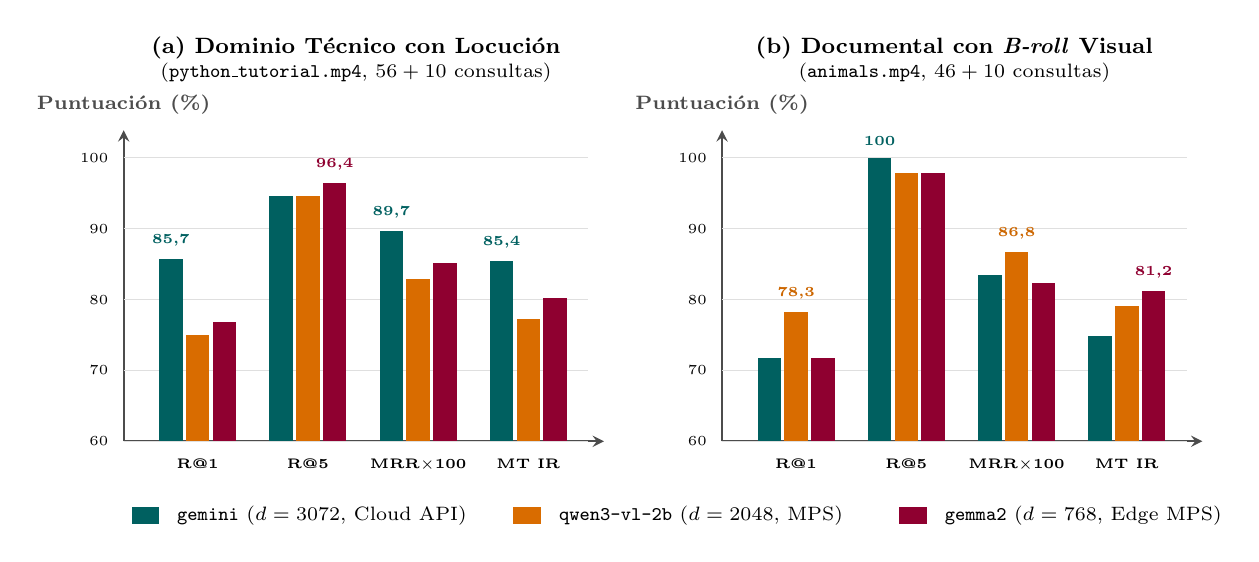
\begin{tikzpicture}
% Panel (a): python_tutorial.mp4
\begin{scope}
\draw[-stealth, thick, black!70] (0,0) -- (6.1,0);
\draw[-stealth, thick, black!70] (0,0) -- (0,3.95) node[above=2pt, font=\scriptsize\bfseries] {Puntuación (\%)};

% Líneas horizontales 60% a 100% (escala: (v - 60) * 0.09 cm)
\foreach \y/\lab in {0.0/60, 0.9/70, 1.8/80, 2.7/90, 3.6/100} {
    \draw[gray!25, thin] (0,\y) -- (5.9,\y);
    \node[left=2pt, font=\tiny] at (0,\y) {\lab};
}

% Grupo R@1 (x ~ 0.9), R@5 (x ~ 2.3), MRR (x ~ 3.7), MT IR (x ~ 5.1)
% Barras ancho 0.30, separacion 0.34
% Gemini (teal), Qwen (orange), Gemma (purple)
\fill[teal!75!black]    (0.45,0) rectangle (0.75,2.314);
\fill[orange!85!black]  (0.79,0) rectangle (1.09,1.350);
\fill[purple!75!black]  (1.13,0) rectangle (1.43,1.511);
\node[above=1pt, font=\tiny\bfseries, teal!75!black] at (0.60,2.314) {85,7};

\fill[teal!75!black]    (1.85,0) rectangle (2.15,3.118);
\fill[orange!85!black]  (2.19,0) rectangle (2.49,3.118);
\fill[purple!75!black]  (2.53,0) rectangle (2.83,3.279);
\node[above=1pt, font=\tiny\bfseries, purple!75!black] at (2.68,3.279) {96,4};

\fill[teal!75!black]    (3.25,0) rectangle (3.55,2.676);
\fill[orange!85!black]  (3.59,0) rectangle (3.89,2.060);
\fill[purple!75!black]  (3.93,0) rectangle (4.23,2.261);
\node[above=1pt, font=\tiny\bfseries, teal!75!black] at (3.40,2.676) {89,7};

\fill[teal!75!black]    (4.65,0) rectangle (4.95,2.288);
\fill[orange!85!black]  (4.99,0) rectangle (5.29,1.550);
\fill[purple!75!black]  (5.33,0) rectangle (5.63,1.825);
\node[above=1pt, font=\tiny\bfseries, teal!75!black] at (4.80,2.288) {85,4};

\node[below=3pt, font=\tiny\bfseries] at (0.94,0) {R@1};
\node[below=3pt, font=\tiny\bfseries] at (2.34,0) {R@5};
\node[below=3pt, font=\tiny\bfseries] at (3.74,0) {MRR$\times$100};
\node[below=3pt, font=\tiny\bfseries] at (5.14,0) {MT IR};

\node[font=\footnotesize\bfseries, align=center] at (2.95,4.85) {(a) Dominio Técnico con Locución\\[-1pt]{\scriptsize\normalfont(\texttt{python\_tutorial.mp4}, $56+10$ consultas)}};
\end{scope}

% Panel (b): animals.mp4
\begin{scope}[xshift=7.6cm]
\draw[-stealth, thick, black!70] (0,0) -- (6.1,0);
\draw[-stealth, thick, black!70] (0,0) -- (0,3.95) node[above=2pt, font=\scriptsize\bfseries] {Puntuación (\%)};

\foreach \y/\lab in {0.0/60, 0.9/70, 1.8/80, 2.7/90, 3.6/100} {
    \draw[gray!25, thin] (0,\y) -- (5.9,\y);
    \node[left=2pt, font=\tiny] at (0,\y) {\lab};
}

\fill[teal!75!black]    (0.45,0) rectangle (0.75,1.057);
\fill[orange!85!black]  (0.79,0) rectangle (1.09,1.643);
\fill[purple!75!black]  (1.13,0) rectangle (1.43,1.057);
\node[above=1pt, font=\tiny\bfseries, orange!80!black] at (0.94,1.643) {78,3};

\fill[teal!75!black]    (1.85,0) rectangle (2.15,3.600);
\fill[orange!85!black]  (2.19,0) rectangle (2.49,3.405);
\fill[purple!75!black]  (2.53,0) rectangle (2.83,3.405);
\node[above=1pt, font=\tiny\bfseries, teal!75!black] at (2.00,3.600) {100};

\fill[teal!75!black]    (3.25,0) rectangle (3.55,2.107);
\fill[orange!85!black]  (3.59,0) rectangle (3.89,2.410);
\fill[purple!75!black]  (3.93,0) rectangle (4.23,2.015);
\node[above=1pt, font=\tiny\bfseries, orange!80!black] at (3.74,2.410) {86,8};

\fill[teal!75!black]    (4.65,0) rectangle (4.95,1.340);
\fill[orange!85!black]  (4.99,0) rectangle (5.29,1.714);
\fill[purple!75!black]  (5.33,0) rectangle (5.63,1.911);
\node[above=1pt, font=\tiny\bfseries, purple!75!black] at (5.48,1.911) {81,2};

\node[below=3pt, font=\tiny\bfseries] at (0.94,0) {R@1};
\node[below=3pt, font=\tiny\bfseries] at (2.34,0) {R@5};
\node[below=3pt, font=\tiny\bfseries] at (3.74,0) {MRR$\times$100};
\node[below=3pt, font=\tiny\bfseries] at (5.14,0) {MT IR};

\node[font=\footnotesize\bfseries, align=center] at (2.95,4.85) {(b) Documental con \textit{B-roll} Visual\\[-1pt]{\scriptsize\normalfont(\texttt{animals.mp4}, $46+10$ consultas)}};
\end{scope}

% Leyenda compartida centrada abajo
\begin{scope}[yshift=-1.05cm, xshift=0.1cm]
\fill[teal!75!black]   (0.0,0) rectangle (0.35,0.22);
\node[right=3pt, font=\scriptsize] at (0.35,0.11) {\texttt{gemini} ($d=3072$, Cloud API)};
\fill[orange!85!black] (4.85,0) rectangle (5.20,0.22);
\node[right=3pt, font=\scriptsize] at (5.20,0.11) {\texttt{qwen3-vl-2b} ($d=2048$, MPS)};
\fill[purple!75!black] (9.75,0) rectangle (10.10,0.22);
\node[right=3pt, font=\scriptsize] at (10.10,0.11) {\texttt{gemma2} ($d=768$, Edge MPS)};
\end{scope}
\end{tikzpicture}
\caption{Comparativa de precisión inter-dominio en dimensión nativa (Etapa 1): \textit{Gemini Embedding 2} lidera el tutorial técnico basado en código y locución sincronizada, pero los modelos locales invierten la jerarquía en metraje documental con \textit{B-roll} visual desacoplado.}
\label{fig:backends_barras_interdominio}
\end{figure}

El análisis conjunto del Cuadro~\ref{tab:backends_metricas_por_dominio} y la Figura~\ref{fig:backends_barras_interdominio} evidencia una clara especialización arquitectónica entre dominios:

\begin{itemize}
    \item \textbf{Superioridad Cloud en discurso técnico estructurado (\texttt{python\_tutorial.mp4}):} \textit{Gemini} ($3072\text{d}$) logra el liderazgo indiscutible en \textit{Recall@1} ($85,71\%$, $+8,92\text{ pp}$ sobre \texttt{gemma2} y $+10,71\text{ pp}$ sobre \texttt{qwen3-vl-2b}) y \textit{MRR} ($0,8973$). Destaca que \texttt{gemma2} ($740\text{M}$ parámetros) supera sistemáticamente a \texttt{qwen3-vl-2b} ($2\text{B}$) en las cuatro métricas del tutorial técnico ($76,79\%$ vs. $75,00\%$ en \textit{Recall@1}; $92,86\%$ vs. $89,29\%$ en \textit{Recall@3}; $96,43\%$ vs. $94,64\%$ en \textit{Recall@5}; y $80,28\%$ vs. $77,22\%$ en \textit{Interval Recall}), lo que indica una alineación lingüística superior del tronco textual \textit{Gemma} frente a términos técnicos de programación en español integrados con la transcripción Whisper.

    \item \textbf{Inversión de rendimiento en metraje visual desacoplado (\texttt{animals.mp4}):} Cuando el audio narrativo describe categorías amplias mientras el fotograma muestra especies concretas, los codificadores visuales abiertos igualan o baten a la API remota. \textbf{\texttt{qwen3-vl-2b} obtiene los mejores registros absolutos del documental} en \textit{Recall@1} ($\mathbf{78,26\%}$, superando en $+6,52\text{ pp}$ a \textit{Gemini} y \textit{Gemma 2}), \textit{Recall@3} ($95,65\%$) y \textit{MRR} ($0,8678$), beneficiándose de su atención nativa sobre teselas visuales M-RoPE de $2\text{B}$ parámetros. Por su parte, \textbf{\texttt{gemma2} encabeza la recuperación multi-objetivo} (\texttt{top\_k=10}), elevando el \textit{Interval Recall} nativo al $\mathbf{81,23\%}$ (y hasta $\mathbf{85,15\%}$ en $512\text{d}/256\text{d}$), más de $10$ puntos porcentuales por encima de \texttt{gemini@3072} ($74,89\%$).

    \item \textbf{Competitividad global agregada ($102$ literales + $20$ multi-objetivo):} Agregando ambos vídeos, el modelo ligero \texttt{gemma2@768} iguala exactamente a \texttt{gemini@3072} tanto en \textit{Recall@3} ($\mathbf{93,14\%}$, $95/102$) como en \textit{Recall@5} ($\mathbf{97,06\%}$, $99/102$), y \texttt{gemma2@512} alcanza el mejor \textit{Interval Recall} multi-objetivo global de todo el estudio ($\mathbf{82,09\%}$ frente a $81,05\%$ de \texttt{gemini@768} y $80,31\%$ de \texttt{qwen3-vl-2b@1536}).
\end{itemize}

\paragraph{Significación Estadística Pareada Inter-Backend (\textit{McNemar} y \textit{Wilcoxon}):}
Los contrastes pareados sobre las puntuaciones por consulta confirman estadísticamente los resultados anteriores: en \texttt{python\_tutorial.mp4} ($N=56$), la ventaja de \texttt{gemini@3072} sobre \texttt{qwen3-vl-2b@2048} alcanza significación nominal en \textit{MRR} ($0,8973$ vs. $0,8289$, $p_{\text{Wilcoxon}} = 0,0396$; \textit{Recall@1} $p_{\text{McNemar}} = 0,1094$), mientras que ninguna otra pareja difiere significativamente ni en Python (\texttt{gemini@3072} vs. \texttt{gemma2@768}: $p_{\text{McNemar}} = 0,1797, p_{\text{Wilcoxon}} = 0,1605$; \texttt{qwen3-vl-2b@2048} vs. \texttt{gemma2@768}: $p_{\text{McNemar}} = 1,0000, p_{\text{Wilcoxon}} = 0,4864$) ni en \texttt{animals.mp4} ($N=46$, todos los contrastes con $p_{\text{McNemar}} \ge 0,5811$ y $p_{\text{Wilcoxon}} \ge 0,4721$). En el agregado global ($N=102$), los dos modelos locales logran \textbf{paridad estadística plena} frente al modelo comercial en la nube tanto en \texttt{qwen3-vl-2b@2048} vs. \texttt{gemini@3072} ($78/102$ vs. $81/102$, $p_{\text{McNemar}} = 0,6776, p_{\text{Wilcoxon}} = 0,2915$) como en \texttt{gemma2@768} vs. \texttt{gemini@3072} ($76/102$ vs. $81/102$, $p_{\text{McNemar}} = 0,3593, p_{\text{Wilcoxon}} = 0,2333$), y en igualdad dimensional entre \texttt{gemini@768} y \texttt{gemma2@768} ($80/102$ vs. $76/102$, $p_{\text{McNemar}} = 0,4807, p_{\text{Wilcoxon}} = 0,2796$).

\subsubsection{Curvas de Ablación Matryoshka (MRL) y Normalización \texorpdfstring{$L_2$}{L2}}
\label{subsubsec:curvas_mrl_normas}

Al evaluar la clase \texttt{Sentence\allowbreak Transformer} mediante el argumento \texttt{truncate\_\allowbreak dim} sobre Apple Silicon (\texttt{bfloat16}), se comprobó un detalle metodológico determinante: \textbf{dicho argumento recorta las primeras $d$ coordenadas sin renormalizar el vector resultante a la hiperesfera unitaria}. El Cuadro~\ref{tab:backends_normas_mrl} documenta las normas $L_2$ observadas tanto en una consulta aislada vía \texttt{truncate\_\allowbreak dim} como sobre los $164$ fragmentos reales de ambos vídeos antes de invocar \texttt{truncate\_\allowbreak and\_\allowbreak normalize\_\allowbreak mrl}.

\begin{table}[htbp]
\centering
\small
\setlength{\tabcolsep}{4.0pt}
\caption{Degradación empírica de la norma euclídea ($L_2$) en prefijos Matryoshka sin renormalizar frente a la restitución unitaria con \texttt{truncate\_and\_normalize\_mrl}.}
\label{tab:backends_normas_mrl}
\begin{adjustbox}{max width=\linewidth}
\begin{tabular}{lcccccc}
\toprule
\textbf{Backend} & \textbf{Dimensión ($d$)} & \textbf{Reducción} & \begin{tabular}[c]{@{}c@{}}\textbf{Norma \texttt{truncate\_dim}}\\\textbf{(consulta en MPS)}\end{tabular} & \begin{tabular}[c]{@{}c@{}}\textbf{Media $\|\mathbf{v}_{1:d}\|_2$}\\\textbf{(164 fragmentos)}\end{tabular} & \begin{tabular}[c]{@{}c@{}}\textbf{Rango $[\min,\max]$}\\\textbf{(164 fragmentos)}\end{tabular} & \begin{tabular}[c]{@{}c@{}}\textbf{Norma tras}\\\textbf{\texttt{truncate\_and\_normalize\_mrl}}\end{tabular} \\
\midrule
\texttt{gemini} & 3072 & $0,0\%$ & - & $1,0000$ & $[1,0000,\; 1,0000]$ & $\mathbf{1,0000}$ \\
\texttt{gemini} & 1536 & $50,0\%$ & - & $0,7267$ & $[0,7235,\; 0,7309]$ & $\mathbf{1,0000}$ \\
\texttt{gemini} & 768 & $75,0\%$ & - & $0,5612$ & $[0,5552,\; 0,5655]$ & $\mathbf{1,0000}$ \\
\midrule
\texttt{qwen3-vl-2b} & 2048 & $0,0\%$ & $1,0004$ & $1,0000$ & $[1,0000,\; 1,0000]$ & $\mathbf{1,0000}$ \\
\texttt{qwen3-vl-2b} & 1536 & $25,0\%$ & $0,8659$ & $0,8666$ & $[0,8450,\; 0,8858]$ & $\mathbf{1,0000}$ \\
\texttt{qwen3-vl-2b} & 768 & $62,5\%$ & $\mathbf{0,6284}$ & $\mathbf{0,6126}$ & $[0,5849,\; 0,6398]$ & $\mathbf{1,0000}$ \\
\midrule
\texttt{gemma2} & 768 & $0,0\%$ & $1,0016$ & $1,0000$ & $[1,0000,\; 1,0000]$ & $\mathbf{1,0000}$ \\
\texttt{gemma2} & 512 & $33,3\%$ & $0,8839$ & $0,8785$ & $[0,8684,\; 0,8854]$ & $\mathbf{1,0000}$ \\
\texttt{gemma2} & 256 & $66,7\%$ & $\mathbf{0,7152}$ & $\mathbf{0,7160}$ & $[0,7003,\; 0,7320]$ & $\mathbf{1,0000}$ \\
\bottomrule
\end{tabular}
\end{adjustbox}
\end{table}

Operar sin renormalizar reduce progresivamente la norma euclídea hasta valores medios de $0,7160$ en \texttt{gemma2@\allowbreak 256} ($0,7152$ en \texttt{truncate\_dim}) y $0,6126$ en \texttt{qwen3-vl-2b@\allowbreak 768} ($0,6284$ en \texttt{truncate\_dim}), distorsionando cualquier cálculo de producto escalar o umbralización fija y debilitando la estabilidad en cuantizaciones futuras (\texttt{int8}). Al delegar el corte en \texttt{truncate\_and\_\allowbreak normalize\_mrl}, todos los vectores recuperan estrictamente $\|\hat{\mathbf{v}}\|_2 = 1,0$.

La Figura~\ref{fig:backends_curvas_mrl} traza las curvas globales de retención Matryoshka sobre las $102$ consultas literales y las $20$ multi-objetivo en función del ahorro efectivo de memoria en Qdrant.

\begin{figure}[htbp]
\centering
\begin{tikzpicture}
% Panel (a): Recall@1 Global (102 consultas) vs Ahorro MRL (%)
\begin{scope}
\draw[-stealth, thick, black!70] (0,0) -- (5.5,0);
\draw[-stealth, thick, black!70] (0,0) -- (0,3.8) node[above=2pt, font=\scriptsize\bfseries] {Recall@1 Global (\%)};

% Eje Y: 70% a 82% -> (v - 70) * 0.28 cm
\foreach \y/\lab in {0.0/70\%, 0.84/73\%, 1.68/76\%, 2.52/79\%, 3.36/82\%} {
    \draw[gray!25, thin] (0,\y) -- (5.2,\y);
    \node[left=2pt, font=\tiny] at (0,\y) {\lab};
}
% Eje X: Ahorro 0% a 80% -> sav * 0.065 cm
\foreach \x/\lab in {0.0/0\%, 1.625/25\%, 3.25/50\%, 4.875/75\%} {
    \draw[gray!30, thin] (\x,0) -- (\x,3.36);
    \node[below=2pt, font=\tiny] at (\x,0) {\lab};
}
\node[below=14pt, font=\scriptsize\bfseries] at (2.6,0) {Ahorro de Almacenamiento (\%)};

% Curva Gemini: (0, 2.635), (3.250, 2.360), (4.875, 2.360)
\draw[very thick, teal!75!black] (0.000,2.635) -- (3.250,2.360) -- (4.875,2.360);
\foreach \x/\y in {0.000/2.635, 3.250/2.360, 4.875/2.360} {
    \fill[teal!75!black] (\x,\y) circle (2.2pt);
}
\node[above right=1pt and 2pt, font=\tiny\bfseries, teal!75!black] at (0.0,2.635) {79,4\% (3072d)};
\node[above=3pt, font=\tiny\bfseries, teal!75!black] at (4.65,2.360) {78,4\% (768d)};

% Curva Qwen3-VL-2B: (0, 1.812), (1.625, 1.812), (4.062, 1.812)
\draw[very thick, orange!85!black] (0.000,1.812) -- (1.625,1.812) -- (4.062,1.812);
\foreach \x/\y in {0.000/1.812, 1.625/1.812, 4.062/1.812} {
    \node[fill=orange!85!black, minimum size=4pt, inner sep=0pt] at (\x,\y) {};
}
\node[above right=2pt and 2pt, font=\tiny\bfseries, orange!80!black] at (0.0,1.812) {76,5\% (2048d $\to$ 768d invariante)};

% Curva Gemma 2: (0, 1.263), (2.164, 1.263), (4.336, 0.988)
\draw[very thick, purple!75!black] (0.000,1.263) -- (2.164,1.263) -- (4.336,0.988);
\foreach \x/\y in {0.000/1.263, 2.164/1.263, 4.336/0.988} {
    \node[regular polygon, regular polygon sides=3, fill=purple!75!black, minimum size=4.6pt, inner sep=0pt] at (\x,\y) {};
}
\node[below right=1pt and 2pt, font=\tiny\bfseries, purple!75!black] at (0.0,1.263) {74,5\% (768d / 512d)};
\node[below=3pt, font=\tiny\bfseries, purple!75!black] at (4.336,0.988) {73,5\% (256d)};

\node[font=\footnotesize\bfseries, align=center] at (2.6,4.75) {(a) Retención \textit{Recall@1} Literal\\[-1pt]{\scriptsize\normalfont(102 consultas agregadas)}};
\end{scope}

% Panel (b): MT Interval Recall Etapa 1 (20 consultas) vs Ahorro MRL (%)
\begin{scope}[xshift=7.7cm]
\draw[-stealth, thick, black!70] (0,0) -- (5.5,0);
\draw[-stealth, thick, black!70] (0,0) -- (0,3.8) node[above=2pt, font=\scriptsize\bfseries] {MT Interval Recall (\%)};

% Eje Y: 75% a 85% -> (v - 75) * 0.336 cm
\foreach \y/\lab in {0.0/75\%, 0.84/77{,}5\%, 1.68/80\%, 2.52/82{,}5\%, 3.36/85\%} {
    \draw[gray!25, thin] (0,\y) -- (5.2,\y);
    \node[left=2pt, font=\tiny] at (0,\y) {\lab};
}
\foreach \x/\lab in {0.0/0\%, 1.625/25\%, 3.25/50\%, 4.875/75\%} {
    \draw[gray!30, thin] (\x,0) -- (\x,3.36);
    \node[below=2pt, font=\tiny] at (\x,0) {\lab};
}
\node[below=14pt, font=\scriptsize\bfseries] at (2.6,0) {Ahorro de Almacenamiento (\%)};

% Curva Gemini: (0, 1.730), (3.250, 1.522), (4.875, 2.033)
\draw[very thick, teal!75!black] (0.000,1.730) -- (3.250,1.522) -- (4.875,2.033);
\foreach \x/\y in {0.000/1.730, 3.250/1.522, 4.875/2.033} {
    \fill[teal!75!black] (\x,\y) circle (2.2pt);
}
\node[above=3pt, font=\tiny\bfseries, teal!75!black] at (4.70,2.033) {81,1\%};

% Curva Qwen3-VL-2B: (0, 1.052), (1.625, 1.784), (4.062, 0.706)
\draw[very thick, orange!85!black] (0.000,1.052) -- (1.625,1.784) -- (4.062,0.706);
\foreach \x/\y in {0.000/1.052, 1.625/1.784, 4.062/0.706} {
    \node[fill=orange!85!black, minimum size=4pt, inner sep=0pt] at (\x,\y) {};
}
\node[below=3pt, font=\tiny\bfseries, orange!80!black] at (4.062,0.706) {77,1\%};
\node[font=\tiny\bfseries, orange!80!black] (qmid) at (2.00,1.12) {80,3\% (1536d)};
\draw[orange!75!black, very thin] (1.625,1.784) -- (qmid.north);

% Curva Gemma 2: (0, 1.932), (2.164, 2.382), (4.336, 1.683)
\draw[very thick, purple!75!black] (0.000,1.932) -- (2.164,2.382) -- (4.336,1.683);
\foreach \x/\y in {0.000/1.932, 2.164/2.382, 4.336/1.683} {
    \node[regular polygon, regular polygon sides=3, fill=purple!75!black, minimum size=4.6pt, inner sep=0pt] at (\x,\y) {};
}
\node[above=3pt, font=\tiny\bfseries, purple!75!black] at (2.164,2.382) {82,1\% (512d)};
\node[above right=2pt and 1pt, font=\tiny\bfseries, purple!75!black] at (0.0,1.932) {80,8\%};

\node[font=\footnotesize\bfseries, align=center] at (2.6,4.75) {(b) \textit{Interval Recall} Multi-Objetivo\\[-1pt]{\scriptsize\normalfont(20 consultas, Etapa 1 \texttt{top\_k=10})}};
\end{scope}

% Leyenda compartida
\begin{scope}[yshift=-1.28cm, xshift=2.2cm]
\draw[very thick, teal!75!black] (0.0,0.1) -- (0.5,0.1);
\fill[teal!75!black] (0.25,0.1) circle (2.2pt);
\node[right=3pt, font=\scriptsize] at (0.5,0.1) {\texttt{gemini}};

\draw[very thick, orange!85!black] (3.4,0.1) -- (3.9,0.1);
\node[fill=orange!85!black, minimum size=4pt, inner sep=0pt] at (3.65,0.1) {};
\node[right=3pt, font=\scriptsize] at (3.9,0.1) {\texttt{qwen3-vl-2b}};

\draw[very thick, purple!75!black] (7.2,0.1) -- (7.7,0.1);
\node[regular polygon, regular polygon sides=3, fill=purple!75!black, minimum size=4.6pt, inner sep=0pt] at (7.45,0.1) {};
\node[right=3pt, font=\scriptsize] at (7.7,0.1) {\texttt{gemma2}};
\end{scope}
\end{tikzpicture}
\caption{Curvas de ablación Matryoshka (MRL) globales: \texttt{qwen3-vl-2b} exhibe invarianza perfecta del $100\%$ en \textit{Recall@1} ($76,5\%$) desde $2048\text{d}$ hasta $768\text{d}$, mientras que \texttt{gemma2@512} alcanza el máximo global de \textit{Interval Recall} multi-objetivo ($82,1\%$) y conserva $73,5\%$ de \textit{Recall@1} incluso a $256\text{d}$ ($1\text{ KB/chunk}$).}
\label{fig:backends_curvas_mrl}
\end{figure}

El análisis de las trayectorias Matryoshka arroja tres resultados notables:
\begin{enumerate}
    \item \textbf{Invarianza en \texttt{qwen3-vl-2b}:} Mantiene exactamente $76,47\%$ ($78/102$) de \textit{Recall@1} y $92,16\%$ ($94/102$) de \textit{Recall@3} en $2048\text{d}$, $1536\text{d}$ y $768\text{d}$ ($-62,5\%$ de espacio), además de mejorar el \textit{Interval Recall} multi-objetivo en $1536\text{d}$ ($80,31\%$ frente a $78,13\%$ en $2048\text{d}$).
    \item \textbf{Eficiencia extrema en \texttt{gemma2@256}:} Con un tamaño de almacenamiento de tan solo $1,00\text{ KB/chunk}$ ($82,00\text{ KB}$ por vídeo frente a $984,00\text{ KB}$ en \texttt{gemini@3072}, una reducción de $12\times$), \texttt{gemma2@256} solo cede un acierto en \textit{Recall@1} respecto a $768\text{d}$ ($75/102$ frente a $76/102$) y conserva $80,01\%$ de \textit{Interval Recall} multi-objetivo.
    \item \textbf{Efecto regularizador en sub-dimensiones intermedias:} Igual que \texttt{gemini} maximiza \textit{Recall@5} ($99,02\%$) y \textit{MT IR} ($81,05\%$) en $768\text{d}$, tanto \texttt{qwen3-vl-2b@1536} como \texttt{gemma2@512} logran sus picos multi-objetivo ($80,31\%$ y $82,09\%$) en dimensión reducida, confirmando que descartar las dimensiones finales de baja varianza mitiga sobreajustes locales en búsquedas de múltiple objetivo.
\end{enumerate}

Desde el punto de vista inferencial ($N=102$), la compresión desde la dimensión nativa hasta la mínima evaluada en cada motor no produce pérdida estadísticamente significativa ni en \textit{Recall@1} ni en \textit{MRR}: \texttt{gemini} ($3072\text{d} \to 768\text{d}$: $p_{\text{McNemar}} = 1,0000, p_{\text{Wilcoxon}} = 0,6729$), \texttt{qwen3-vl-2b} ($2048\text{d} \to 768\text{d}$: $p_{\text{McNemar}} = 1,0000, p_{\text{Wilcoxon}} = 0,5519$) y \texttt{gemma2} ($768\text{d} \to 256\text{d}$: $p_{\text{McNemar}} = 1,0000, p_{\text{Wilcoxon}} = 0,4370$).

\subsubsection{Rendimiento Computacional, Latencia y Huella de Memoria}
\label{subsubsec:rendimiento_memoria_backends}

El Cuadro~\ref{tab:backends_coste_recursos} consolida los costes de indexación, tiempos de respuesta en consulta y consumo máximo de memoria RAM (\texttt{RSS}) y gráfica integrada (\texttt{MPS driver\_allocated\_memory}), complementado visualmente por la Figura~\ref{fig:backends_tradeoff_latencia_memoria}.

\begin{table}[htbp]
\centering
\small
\setlength{\tabcolsep}{3.5pt}
\caption{Rendimiento computacional, latencia de consulta y huella máxima de memoria por vídeo y backend (configuraciones nativas).}
\label{tab:backends_coste_recursos}
\begin{adjustbox}{max width=\linewidth}
\begin{tabular}{llccccccc}
\toprule
\textbf{Corpus} & \textbf{Backend (Dim)} & \textbf{Dispositivo} & \begin{tabular}[c]{@{}c@{}}\textbf{Indexación}\\\textbf{Total}\end{tabular} & \begin{tabular}[c]{@{}c@{}}\textbf{Coste /}\\\textbf{Fragmento}\end{tabular} & \begin{tabular}[c]{@{}c@{}}\textbf{Consulta}\\\textbf{Media (ms)}\end{tabular} & \begin{tabular}[c]{@{}c@{}}\textbf{Consulta}\\\textbf{Mediana (ms)}\end{tabular} & \begin{tabular}[c]{@{}c@{}}\textbf{Pico RSS}\\\textbf{(MB)}\end{tabular} & \begin{tabular}[c]{@{}c@{}}\textbf{Pico MPS}\\\textbf{(MB)}\end{tabular} \\
\midrule
\multirow{3}{*}{\texttt{python\_tutorial.mp4}}
 & \texttt{gemini} ($3072$) & Cloud API & $227,31\text{ s}$ & $2,772\text{ s}$ & $484,67$ & $481,30$ & $391,4$ & $0$ \\
 & \texttt{qwen3-vl-2b} ($2048$) & Local MPS & $\mathbf{142,23\text{ s}}$ & $\mathbf{1,734\text{ s}}$ & $95,11$ & $97,69$ & $2.095,1$ & $4.736,5$ \\
 & \texttt{gemma2} ($768$) & Local MPS & $247,73\text{ s}$ & $3,021\text{ s}$ & $\mathbf{30,11}$ & $\mathbf{29,93}$ & $3.081,5$ & $\mathbf{2.552,6}$ \\
\midrule
\multirow{3}{*}{\texttt{animals.mp4}}
 & \texttt{gemini} ($3072$) & Cloud API & $187,12\text{ s}$ & $2,282\text{ s}$ & $1.086,72^*$ & $464,18$ & $424,0$ & $0$ \\
 & \texttt{qwen3-vl-2b} ($2048$) & Local MPS & $\mathbf{126,05\text{ s}}$ & $\mathbf{1,537\text{ s}}$ & $92,33$ & $90,94$ & $1.995,8$ & $4.737,7$ \\
 & \texttt{gemma2} ($768$) & Local MPS & $245,49\text{ s}$ & $2,994\text{ s}$ & $\mathbf{31,08}$ & $\mathbf{30,20}$ & $2.641,2$ & $\mathbf{2.592,1}$ \\
\bottomrule
\end{tabular}
\end{adjustbox}
\vspace{2pt}
{\scriptsize $^*$Incluye picos puntuales de latencia TLS/API remota; la mediana ($464,18\text{ ms}$) representa el tiempo típico de respuesta en red.}
\end{table}

\begin{figure}[htbp]
\centering
\begin{tikzpicture}
% Panel (a): Latencia consulta mediana (ms) vs Coste indexacion (s/chunk)
\begin{scope}
\draw[-stealth, thick, black!70] (0,0) -- (5.5,0);
\draw[-stealth, thick, black!70] (0,0) -- (0,3.8) node[above=2pt, font=\scriptsize\bfseries] {Indexación (s/chunk)};

% Y: 0 a 3.5 s/chunk (escala 1.0 cm por s/chunk)
\foreach \y/\lab in {1.0/1{,}0, 2.0/2{,}0, 3.0/3{,}0} {
    \draw[gray!25, thin] (0,\y) -- (5.3,\y);
    \node[left=2pt, font=\tiny] at (0,\y) {\lab};
}
% X: 0 a 550 ms (escala 0.01 cm/ms)
\foreach \x/\lab in {1.0/100, 2.5/250, 4.0/400, 5.0/500} {
    \draw[gray!25, thin] (\x,0) -- (\x,3.5);
    \node[below=2pt, font=\tiny] at (\x,0) {\lab};
}
\node[below=14pt, font=\scriptsize\bfseries] at (2.7,0) {Mediana Consulta (ms)};

% Zona optima Pareto esquina inferior izquierda
\fill[green!12, rounded corners=3pt] (0.05,0.05) rectangle (1.45,1.95);
\node[font=\tiny\itshape, green!50!black] at (0.75,0.30) {Frente local rápido};

% Gemma2: Py (0.299, 3.021), An (0.302, 2.994)
\node[regular polygon, regular polygon sides=3, fill=purple!75!black, minimum size=5pt, inner sep=0pt] (gpy) at (0.299,3.021) {};
\node[regular polygon, regular polygon sides=3, draw=purple!75!black, fill=white, thick, minimum size=5pt, inner sep=0pt] (gan) at (0.302,2.994) {};
\node[right=4pt, font=\tiny\bfseries, purple!75!black, align=left] at (0.35,3.05) {\texttt{gemma2}\\($\sim 30\text{ ms}$, $3,0\text{ s/c}$)};

% Qwen: Py (0.977, 1.734), An (0.909, 1.537)
\node[fill=orange!85!black, minimum size=4.5pt, inner sep=0pt] (qpy) at (0.977,1.734) {};
\node[draw=orange!85!black, fill=white, thick, minimum size=4.5pt, inner sep=0pt] (qan) at (0.909,1.537) {};
\node[right=4pt, font=\tiny\bfseries, orange!80!black, align=left] at (1.05,1.65) {\texttt{qwen3-vl-2b}\\($91$--$98\text{ ms}$, $1,5$--$1,7\text{ s/c}$)};

% Gemini: Py (4.813, 2.772), An (4.642, 2.282)
\fill[teal!75!black] (4.813,2.772) circle (2.4pt);
\draw[teal!75!black, fill=white, thick] (4.642,2.282) circle (2.4pt);
\node[left=4pt, font=\tiny\bfseries, teal!75!black, align=right] at (4.60,2.55) {\texttt{gemini} Cloud\\($464$--$481\text{ ms}$, $2,3$--$2,8\text{ s/c}$)};

\node[font=\footnotesize\bfseries, align=center] at (2.7,4.75) {(a) Latencia de Consulta vs. Indexación\\[-1pt]{\scriptsize\normalfont(Símbolo sólido: Python; hueco: Animals)}};
\end{scope}

% Panel (b): Pico de Memoria RSS vs GPU Metal (MPS)
\begin{scope}[xshift=7.8cm]
\draw[-stealth, thick, black!70] (0,0) -- (5.3,0);
\draw[-stealth, thick, black!70] (0,0) -- (0,3.8) node[above=2pt, font=\scriptsize\bfseries] {Memoria Pico (MB)};

% Escala Y: 1 cm = 1500 MB (hasta 5000 MB -> 3.33 cm)
\foreach \y/\lab in {1.0/1.500, 2.0/3.000, 3.0/4.500} {
    \draw[gray!25, thin] (0,\y) -- (5.1,\y);
    \node[left=2pt, font=\tiny] at (0,\y) {\lab};
}

% Grupo Gemini (x=0.8), Qwen (x=2.4), Gemma (x=4.0), media Py/An:
% Gemini: RSS=408 (0.272), MPS=0
\fill[blue!70!black] (0.50,0) rectangle (0.90,0.272);
\fill[magenta!75!black] (0.94,0) rectangle (1.34,0.020);
\node[above=1pt, font=\tiny\bfseries, blue!70!black] at (0.68,0.272) {408};
\node[above=1pt, font=\tiny, magenta!75!black] at (1.14,0.03) {0};

% Qwen: RSS=2045 (1.363), MPS=4737 (3.158)
\fill[blue!70!black] (2.10,0) rectangle (2.50,1.363);
\fill[magenta!75!black] (2.54,0) rectangle (2.94,3.158);
\node[above=1pt, font=\tiny\bfseries, blue!70!black] at (2.22,1.363) {2.045};
\node[above=1pt, font=\tiny\bfseries, magenta!75!black] at (2.74,3.158) {4.737};

% Gemma2: RSS=2861 (1.908), MPS=2572 (1.715)
\fill[blue!70!black] (3.70,0) rectangle (4.10,1.908);
\fill[magenta!75!black] (4.14,0) rectangle (4.54,1.715);
\node[above=1pt, font=\tiny\bfseries, blue!70!black] at (3.82,1.908) {2.861};
\node[above=1pt, font=\tiny\bfseries, magenta!75!black] at (4.42,1.715) {2.572};

\node[below=3pt, font=\scriptsize\bfseries] at (0.92,0) {\texttt{gemini}};
\node[below=3pt, font=\scriptsize\bfseries] at (2.52,0) {\texttt{qwen3-vl-2b}};
\node[below=3pt, font=\scriptsize\bfseries] at (4.12,0) {\texttt{gemma2}};

% Leyenda b
\fill[blue!70!black]    (-0.10,-0.85) rectangle (0.20,-0.65);
\node[right=2pt, font=\tiny] at (0.20,-0.75) {RSS Proceso (promedio)};
\fill[magenta!75!black] (3.00,-0.85) rectangle (3.30,-0.65);
\node[right=2pt, font=\tiny] at (3.30,-0.75) {GPU Driver Metal (MPS)};

\node[font=\footnotesize\bfseries, align=center] at (2.55,4.75) {(b) Huella Física de Memoria\\[-1pt]{\scriptsize\normalfont(Media entre ambos corpus en $16\text{ GB}$)}};
\end{scope}
\end{tikzpicture}
\caption{Compromiso entre rendimiento temporal y recursos de memoria en Apple Silicon M3 ($16\text{ GB}$): \texttt{gemma2} reduce la latencia de consulta local en un factor de $15$--$16\times$ frente a Cloud API consumiendo casi la mitad de memoria MPS que \texttt{qwen3-vl-2b}, mientras que \texttt{qwen3-vl-2b} consigue la indexación de vídeo más veloz.}
\label{fig:backends_tradeoff_latencia_memoria}
\end{figure}

La comparativa temporal y de recursos revela tres hallazgos clave de ingeniería:
\begin{enumerate}
    \item \textbf{Aceleración interactiva de hasta $16\times$ en consultas locales:} Al eliminar el viaje de red HTTP/TLS hasta los servidores de la API Cloud (mediana de $464,18$--$481,30\text{ ms}$), \texttt{qwen3-vl-2b} responde en $90,94$--$97,69\text{ ms}$ ($\approx 5\times$ más rápido) y \texttt{gemma2} en apenas $\mathbf{29,93}$--$\mathbf{30,20\text{ ms}}$ ($15,4\times$--$16,1\times$ más rápido). Esto permite ejecutar búsquedas vectoriales en Qdrant en tiempo casi instantáneo de percepción humana ($< 35\text{ ms}$ totales).
    \item \textbf{Asimetría arquitectónica entre consulta textual e indexación de fotogramas:} Aunque \texttt{gemma2} es $3\times$ más rápido en consultas de texto ($23,6\text{ ms}$ frente a $72,9\text{ ms}$ medidos en aislamiento sobre MPS tras \texttt{torch.mps.synchronize()}), porque en texto puro activa únicamente su tronco lingüístico de $270\text{M}$ parámetros, al indexar fragmentos multimodales de $3$ fotogramas ($512\text{ px}$) invoca su codificador visual ($170\text{M}$) con un coste neto de $1.960,1\text{ ms/chunk}$ frente a $1.180,6\text{ ms/chunk}$ en \texttt{qwen3-vl-2b}. Sumando las etapas constantes de segmentación SSIM y transcripción Whisper, \textbf{\texttt{qwen3-vl-2b} completa la indexación de un vídeo en $126,05$--$142,23\text{ s}$}, superando incluso a \textit{Gemini Cloud} ($187,12$--$227,31\text{ s}$).
    \item \textbf{Contención en $16\text{ GB}$ unificados:} Al combinar la descarga de Whisper con \texttt{Semaphore(1)}, ningún motor local bloquea el equipo: \texttt{gemma2} opera con apenas $\mathbf{2,55\text{--}2,59\text{ GB}}$ \textbf{de memoria GPU Metal} ($46\%$ menos que \texttt{qwen3-vl-2b}, con $4,74\text{ GB}$), posicionándose como la alternativa óptima para portátiles o despliegue en el borde con restricciones estrictas de VRAM compartida.
\end{enumerate}

\subsubsection{Criterios de Selección Arquitectónica Cloud vs. Local}
A la luz de la evidencia recopilada en ambos vídeos, no existe un ganador absoluto en todas las dimensiones operativas, sino un espectro complementario claro:
\begin{itemize}
    \item \textbf{Escenarios sin GPU o de discurso técnico denso:} \texttt{gemini@768} mantiene el mejor equilibrio global de precisión en Etapa 1 en contenido hablado/código ($85,71\%$ \textit{Recall@1} en Python) con huella local prácticamente nula ($391-424\text{ MB}$ RSS), a costa de $464-481\text{ ms}$ de red y sujeción a cuotas RPD.
    \item \textbf{Búsqueda visual en metraje documental o alta velocidad de ingesta privada:} \texttt{qwen3-vl-2b@\allowbreak 1536} ofrece la mejor combinación de precisión puramente visual ($78,26\%$ \textit{Recall@1} y $81,31\%$ \textit{MT IR} en \texttt{animals.mp4}) y el menor tiempo de indexación ($1,54-1,73\text{ s/chunk}$) sin cuotas externas, asumiendo $\approx 4,74\text{ GB}$ de memoria Metal.
    \item \textbf{Computación Edge, baja latencia y mínimo almacenamiento:} Las variantes \texttt{gemma2@\allowbreak 512} y \texttt{gemma2@\allowbreak 256} ejecutan consultas locales en $\approx 30\text{ ms}$ consumiendo solo $2,55-2,59\text{ GB}$ de MPS, lideran el \textit{Interval Recall} multi-objetivo global ($82,09\%$ en $512\text{d}$) y reducen la base vectorial hasta $1,00\text{ KB/chunk}$ ($82\text{ KB}$ por vídeo).
\end{itemize}
